
\pagestyle{empty}
\usepackage[a4paper,top=2cm,bottom=2cm,left=1.5cm,right=1.5cm]{geometry}

%\setlength{\textheight}{250mm}
%\setlength{\textwidth}{180mm}
%\setlength{\oddsidemargin}{-8mm}
%\setlength{\topmargin}{-1.5cm}

\usepackage{amsmath}
\usepackage{amsthm}
\usepackage{psfrag}
\usepackage{graphicx}
\usepackage{bm}
\usepackage{mathrsfs}
\usepackage{icomma} % pacchetto per limitare lo spazio standard posto dopo la virgola in caso che la virgola sia tra cifre
\usepackage{amsfonts} % amplia i caratteri matematici disponibili
\usepackage{amssymb}
%\usepackage{wrapfig}
\usepackage{empheq}

\usepackage{epstopdf}
\usepackage[utf8x]{inputenc}
\usepackage{ifthen}

\usepackage{caption}

\usepackage[italian]{babel}
%\usepackage[latin1]{inputenc}

\usepackage{subfig}

\usepackage{pgfplots}
\pgfplotsset{compat=1.9}
\usepackage{hyperref}

\input{def}

\newcommand{\kg}{\textrm{kg}}
\newcommand{\K}{\textrm{K}}
\newcommand{\m} {\textrm{m}}
\newcommand{\dm}{\textrm{dm}}
\newcommand{\cm}{\textrm{cm}}
\newcommand{\mm}{\textrm{mm}}
\newcommand{\s} {\textrm{s}}
\newcommand{\N} {\textrm{N}}
\renewcommand{\Pa}{\textrm{Pa}}
%\newtheorem{exerciseS}{Esercizio}[section]

%% ###########################################################
\def \flagSect{0} % 1    : numerazione
		  % else : niente
%\newcommand{\taitol}[1]  % stile titolo
%{
%%{\textit{#1}}
%{#1}
%}
\def \soluzione{Soluzione}
\def \partePrima{Concetti. }
\def \parteSeconda{Svolgimento. }
%\def \parteTerza{}
\newcommand{\sol}{\subsubsection*{\soluzione}}
\newcommand{\partone}{\ \ \ \ \ \textbf{\partePrima}}
\newcommand{\parttwo}{\vspace{0.2cm}\textbf{\parteSeconda}}

\ifnum\flagSect=1
\newtheorem{esercizio}{Esercizio}%[section]
\else
\newtheorem*{esercizio}{Esercizio}
\fi

\newtheorem*{teorema}{Teorema}
\newtheorem*{lemma}{Lemma}

% ###########################################################
%\def \flagSect{0} % 1    : numerazione
		  % else : niente
%\newcommand{\taitol}[1]  % stile titolo
%{
%%{\textit{#1}}
%{#1}
%}
\def \soluzione{Soluzione}
\def \partePrima{Concetti. }
\def \parteSeconda{Svolgimento. }
%\def \parteTerza{}
\newcommand{\sol}{\subsubsection*{\soluzione}}
\newcommand{\partone}{\ \ \ \ \ \textbf{\partePrima}}
\newcommand{\parttwo}{\vspace{0.2cm}\textbf{\parteSeconda}}

\ifnum\flagSect=1
\newtheorem{esercizio}{Esercizio}%[section]
\else
\newtheorem*{esercizio}{Esercizio}
\fi

\newtheorem*{teorema}{Teorema}
\newtheorem*{lemma}{Lemma}

% ###########################################################
%\def \flagSect{0} % 1    : numerazione
		  % else : niente
%\newcommand{\taitol}[1]  % stile titolo
%{
%%{\textit{#1}}
%{#1}
%}
\def \soluzione{Soluzione}
\def \partePrima{Concetti. }
\def \parteSeconda{Svolgimento. }
%\def \parteTerza{}
\newcommand{\sol}{\subsubsection*{\soluzione}}
\newcommand{\partone}{\ \ \ \ \ \textbf{\partePrima}}
\newcommand{\parttwo}{\vspace{0.2cm}\textbf{\parteSeconda}}

\ifnum\flagSect=1
\newtheorem{esercizio}{Esercizio}%[section]
\else
\newtheorem*{esercizio}{Esercizio}
\fi

\newtheorem*{teorema}{Teorema}
\newtheorem*{lemma}{Lemma}

% ###########################################################
%\input{logicNumb}
%\newcommand{\sectionIf}[2]
%{
%   \ifthenelse{\equal{#1}{1}}
%              {\subsection{#2}}{\subsection*{#2}}
%}
% ###########################################################

%\newcommand{\sectionIf}[2]
%{
%   \ifthenelse{\equal{#1}{1}}
%              {\subsection{#2}}{\subsection*{#2}}
%}
% ###########################################################

%\newcommand{\sectionIf}[2]
%{
%   \ifthenelse{\equal{#1}{1}}
%              {\subsection{#2}}{\subsection*{#2}}
%}
% ###########################################################

%\newcommand{\sectionIf}[2]
%{
%   \ifthenelse{\equal{#1}{1}}
%              {\subsection{#2}}{\subsection*{#2}}
%}
%% ###########################################################


\begin{document}

%% ###########################################################
\noindent
\begin{tabular}{cc}
\begin{minipage}{0.60\textwidth}
\begin{exerciseS}
Si consideri la corrente piana fra due cilindri coassiali rotanti.
Si misura la velocit\`a in due punti posti rispettivamente a $1/4$ e 
$3/4$ del gap fra i due cilindri: 
$u_{\theta,1/4} = 0.5\, \m/\s$, 
$u_{\theta,3/4} = 0.8\, \m/\s$.
Si determini la velocit\`a di rotazione dei due cilindri nonch\'e
la pressione in corrispondenza del cilindro interno sapendo che
la pressione in corrispondenza del cilindro esterno vale $5\, \Pa$,
che la densit\`a del fluido \`e pari a $1.225\, \kg/\m^3$,
che il diametro del cilindro interno \`e $d =0.1 \,\m$ e che il diametro 
del cilindro esterno \`e $D = 0.16 \, \m$.
 
($\Omega_{in}=6.663\, {\rm s^{-1}}$, $\Omega_{ext}=11.743\, {\rm s^{-1}}$)
\end{exerciseS}
\end{minipage}
&
\begin{minipage}{0.35\textwidth}
   \begin{center}
   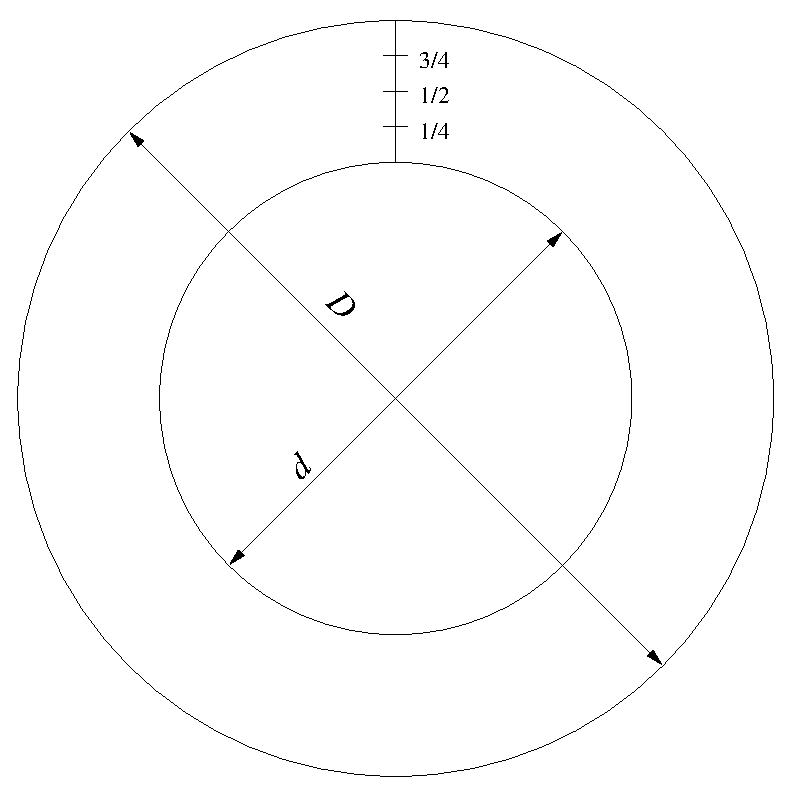
\includegraphics[width=0.70\textwidth]{./06SlnEsatte/cilindri_coax.eps}
   \end{center}
\end{minipage}
\end{tabular}

\vspace{1cm}

%% ###########################################################
\noindent
\begin{tabular}{cc}
\begin{minipage}{0.60\textwidth}
\begin{exerciseS}
Una lastra piana di lunghezza e apertura infinita si spessore 
$t=1\, {\rm mm}$ scorre in un canale piano di altezza $H=2.22\, {\rm mm}$
contenente acqua in condizioni standard. 
Essa viene mantenuta a distanza costante $h_1=0.5\, {\rm mm}$ dalla parete
superiore e si muove a velocit\`a constante $U=0.55 \, {\rm m/s}$.

Calcolare:
\begin{itemize}
\item il numero di Reynolds basato sulla velocit\`a $U$ della parete
e sulla distanza fra le pareti sia per la porzione di corrente superiore
sia per quella inferiore;
\item la componente orizzontale del risultante delle forze per unit\`a di
superficie esercitate dal fluido sulla lamina;
\item la potenza per unit\`a di superficie che occorre fornire alla 
lastra per mantenerla in moto uniforme.
\end{itemize}

(${\rm Re_{sup}}=239$, 
 ${\rm Re_{inf}}=344$, 
 $F_x=-2.14\, {\rm N/m^2}$, 
 $P=1.17\, {\rm W/m^2}$)
\end{exerciseS}
\end{minipage}
&
\begin{minipage}{0.35\textwidth}
   \begin{center}
   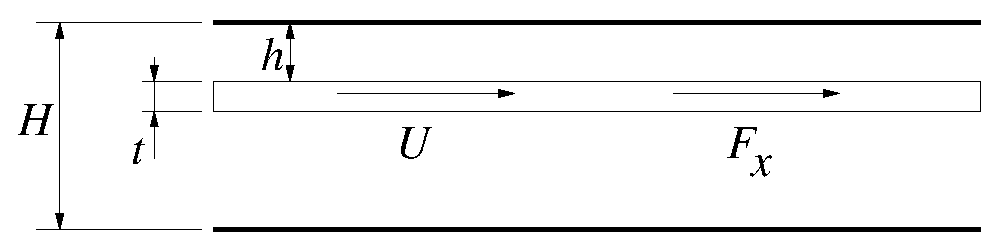
\includegraphics[width=0.70\textwidth]{./06SlnEsatte/lastracanale.eps}
   \end{center}
\end{minipage}
\end{tabular}

\vspace{1cm}

%% ###########################################################
\noindent
\begin{tabular}{cc}
\begin{minipage}[b]{0.95\textwidth}
\begin{exerciseS}
Si consideri una corrente d'acqua a pelo libero, laminare e stazionaria, che
scorre su una parete verticale piana di lunghezza e apertura infinita.
Si ipotizzi che la pressione atmosferica che agisce sul pelo libero sia
uniforme. Si ipotizzi inoltre che lo sforzo tangenziale fra acqua e aria in
corrispondenza del pelo libero sia nullo.

Assegnata la portata in massa per unit\`a di apertura 
$\overline{Q}=0.5\, {\rm kg/(ms)}$, determinare
\begin{enumerate}
  \item lo spessore $h$ della corrente d'acqua;
  \item lo sforzo tangenziale a parete;
  \item la velocit\`a in corrispondenza del pelo libero;
  \item la velocit\`a media e il numero di Reynolds basato su tale velocit\`a
        media e sullo spessore della corrente.
\end{enumerate}
Si sostituisca poi al pelo libero una parete solida.
Si determini quale dovrebbe essere la velocit\`a di tale parete per ottenere
una portata nulla.

Dati: $\overline{\rho}= 999\, {\rm kg/m^3}$, 
$\overline{\mu}= 1.15\, 10^{-3}{\rm kg/(ms)}$.

($h=5.61\, 10^{-4}\, {\rm m}$, $\tau = 5.494\, {\rm Pa}$, $u(h)=1.339\, {\rm m/s}$,
$\overline{U}=0.893\, {\rm m/s}$, ${\rm Re}=434.8$, $U=-0.4464\, {\rm m/s}$.)
\end{exerciseS}
\end{minipage}
\end{tabular}

\vspace{1cm}

%% ###########################################################
\noindent
\begin{tabular}{cc}
\begin{minipage}[b]{0.60\textwidth}
\begin{exerciseS}
\`E dato un canale piano, di lunghezza e apertura infinita, 
orizzontale, di altezza $H=1.51\,{\rm mm}$,
delimitato da una parete inferiore fissa e da una parete superiore 
mobile con velocit\`a orizzontale, costante e positiva $U=0.31\,{\rm m/s}$.
Il canale contiene acqua in condizioni standard.

Per quale condizione la portata nel canale risulta nulla?


(${\rm Re}=441$, $G_p= 930\, {\rm Pa/m}$)
\end{exerciseS}
\end{minipage}
&
\begin{minipage}[b]{0.35\textwidth}
   \begin{center}
   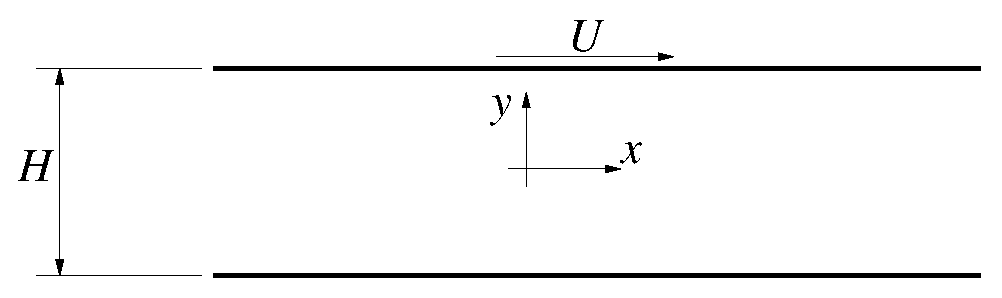
\includegraphics[width=0.90\textwidth]{./06SlnEsatte/canalepiano.eps}
   \end{center}
\end{minipage}
\end{tabular}

\vspace{1cm}

%% ###########################################################
\noindent
\begin{tabular}{cc}
\begin{minipage}[b]{0.60\textwidth}
\begin{exerciseS}
Un manometro a mercurio ($\rho_{\rm hg} = 13610 \, {\rm kg/m^3}$)
collega due prese di pressione posizionate a una distanza di $l = 2 \,
\rm{m}$ l'una dall'altra lungo un tubo orizzontale di diametro $2R = 5 \,
{\rm cm}$ in cui scorre un fluido con densità $\rho_{\rm f} = 950 \, {\rm
kg/m^3}$. Se la differenza fra le altezze dei peli liberi del 
liquido manometrico nelle due colonne
vale $\Delta h = 4 \, \rm{cm}$ e la portata volumetrica che scorre nel tubo è 
$Q= 6\, \rm{m^3/s}$,
quanto valgono la viscosità $\mu$ del fluido e lo sforzo a parete
$\tau_w$?

($\mu = 6.36\,10^{-5} \, \rm{Kg/(m\, s)}$,
$\tau_w = 31.05\, \zb\, \rm{N/m^2}$)
\end{exerciseS}
\end{minipage}
&
\begin{minipage}[b]{0.35\textwidth}
   \begin{center}
   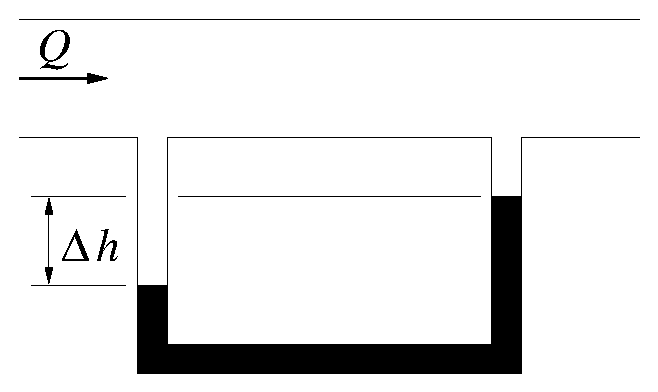
\includegraphics[width=0.70\textwidth]{./06SlnEsatte/poiseuille.eps}
   \end{center}
\end{minipage}
\end{tabular}

\vspace{1cm}

%% ###########################################################
\noindent
\begin{tabular}{cc}
\begin{minipage}{0.60\textwidth}
\begin{exerciseS}
Si consideri la corrente piana fra due cilindri coassiali di raggio $R_1$ e $R_2$.
Il cilindro esterno è fermo, mentre quello interno è messo in rotazione da
 un motore con curva caratteristica $C(\Omega) = \alpha - \beta \Omega$.
Si determini il punto di equilibrio del sistema ($\Omega$ costante).
Si determini inoltre la pressione in corrispondenza del cilindro interno sapendo che
la pressione in corrispondenza del cilindro esterno vale $5\, \Pa$.
La densit\`a del fluido \`e pari a $1.225\, \kg/\m^3$,
che il diametro del cilindro interno \`e $d =0.1 \,\m$ e che il diametro 
del cilindro esterno \`e $D = 0.16 \, \m$.
 
($\Omega_{in}=6.663\, {\rm s^{-1}}$, $\Omega_{ext}=11.743\, {\rm s^{-1}}$)
\end{exerciseS}
\end{minipage}
&
\begin{minipage}{0.35\textwidth}
   \begin{center}
   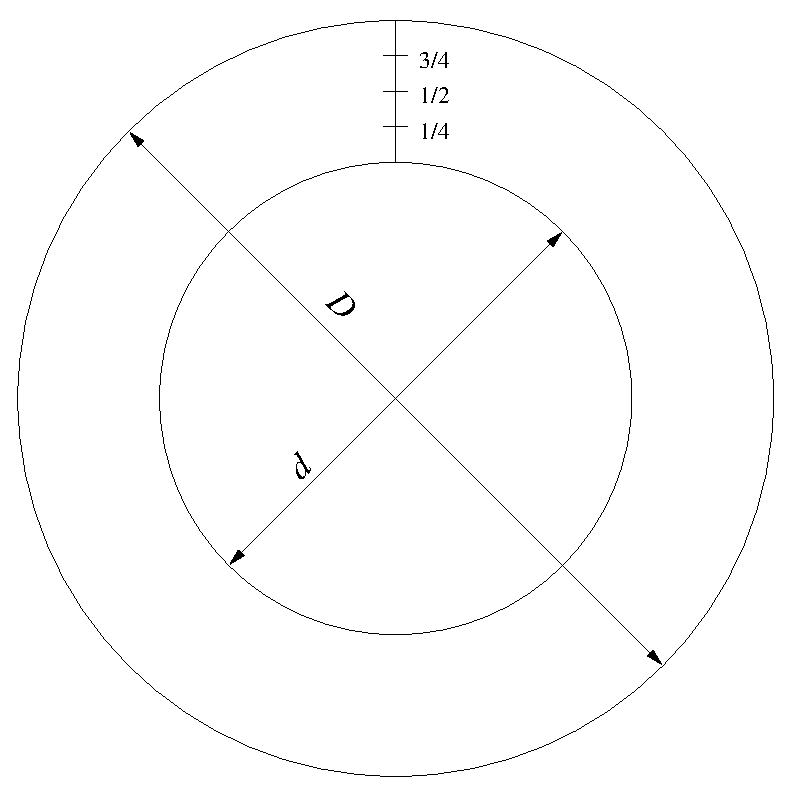
\includegraphics[width=0.70\textwidth]{./06SlnEsatte/cilindri_coax.eps}
   \end{center}
\end{minipage}
\end{tabular}

\vspace{1cm}

%% ###########################################################
\begin{exerciseS}
 Si proponga un modo per determinare sperimentalmente la viscosità di un fluido e si
 discutano le ipotesi alle basi di tale metodo e i suoi limiti.
\end{exerciseS}



\end{document}
